\documentclass[12pt]{article}
\usepackage[margin=1in]{geometry}
\usepackage{amsmath,amssymb,amsthm,booktabs,array}
\usepackage{microtype}
\usepackage{newcomputermodern}
\usepackage[most]{tcolorbox}
\usepackage{tikz}
\usetikzlibrary{arrows.meta,positioning}
\usepackage[hidelinks]{hyperref}
\usepackage{enumitem,needspace}
\setcounter{tocdepth}{1}
\AddToHook{cmd/section/before}{\Needspace{7\baselineskip}}
\AddToHook{cmd/subsection/before}{\Needspace{5\baselineskip}}
\setlist{itemsep=2pt,topsep=4pt}
\newtcolorbox{remarkbox}[1][Note]{colback=gray!5,colframe=gray!60,title={#1},fonttitle=\bfseries,arc=2mm,boxrule=.6pt,breakable}
\newtcolorbox{correction}[1][Correction]{colback=red!3,colframe=red!55!black,title={#1},fonttitle=\bfseries,arc=2mm,boxrule=.6pt,breakable}
\newtcolorbox{todo}[1][TODO from the manuscript]{colback=yellow!8,colframe=orange!70!black,title={#1},fonttitle=\bfseries,arc=2mm,boxrule=.6pt,breakable}
\newtcolorbox{supplement}[1][Lecture supplement]{colback=blue!3,colframe=blue!50!black,title={#1},fonttitle=\bfseries,arc=2mm,boxrule=.6pt,breakable}
\newcommand{\E}{\mathbb E}
\newcommand{\Prob}{\mathbb P}
\newcommand{\Var}{\operatorname{Var}}
\newcommand{\Cov}{\operatorname{Cov}}
\newcommand{\pa}{\operatorname{Pa}}
\newcommand{\de}{\operatorname{De}}
\newcommand{\an}{\operatorname{An}}
\newcommand{\nd}{\operatorname{Nd}}
\newcommand{\doo}{\operatorname{do}}
\newcommand{\ind}{\mathrel{\perp\!\!\!\perp}}
\newcommand{\nind}{\mathrel{\not\!\perp\!\!\!\perp}}
\newcommand{\dsep}{\mathrel{\perp\!\!\!\perp}_{d}}
\newcommand{\source}[1]{\par\smallskip{\small\color{gray!80!black}\textit{Manuscript: #1.}}\par}
\setlength{\parindent}{0pt}
\setlength{\parskip}{6pt}
\setlength{\emergencystretch}{2em}
\tikzset{v/.style={circle,draw=blue!45!black,fill=blue!3,minimum size=8mm,inner sep=2pt},edge/.style={-{Stealth[length=2mm]},thick}}
\author{Liang-Cheng Chen}
\date{Spring 2026\quad /\quad Typeset October 25, 2026}
% TASK.md explicitly requests double-dollar delimiters for INLINE math.
% Make the dollar character active so paired $$...$$ means ensuremath,
% not TeX display math. Display formulas use equation/align exclusively.
\catcode`\$=\active
\protected\long\def$$#1$${\ensuremath{#1}}

\title{STAT 566: Causal Modeling\\[.4em]\large Note 5: Instrumental Variables and Mendelian Randomization}
\begin{document}
\maketitle
\begin{remarkbox}[Reading guide]
English transcription and edited study notes. Yellow boxes preserve manuscript TODOs; red boxes explain corrections; blue boxes identify lecture-based additions. Gray boxes clarify questions. Source-page markers refer to the original handwritten PDF, not this edition.
\end{remarkbox}
\tableofcontents
\clearpage
\section{Why instrumental variables?}
\source{stat566-note5, p. 1 (May 19); Lecture 8, Section 1}
When an unmeasured $$U$$ causes both treatment $$A$$ and outcome $$Y$$, observed covariate adjustment may not identify the effect. An instrument $$I$$ supplies variation in treatment unrelated to the latent confounding mechanism:
\begin{center}
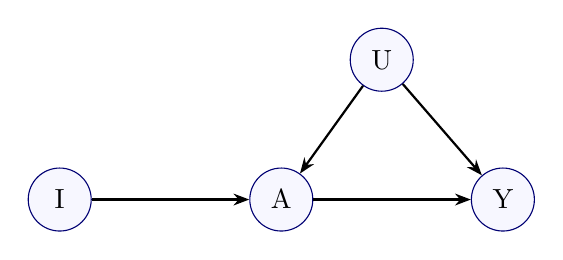
\begin{tikzpicture}[node distance=20mm]
\node[v] (i) {I};\node[v,right=of i] (a) {A};\node[v,right=of a] (y) {Y};\node[v,above right=12mm and 7mm of a] (u) {U};
\draw[edge] (i)--(a);\draw[edge] (a)--(y);\draw[edge] (u)--(a);\draw[edge] (u)--(y);
\end{tikzpicture}
\end{center}
The core linear IV assumptions are:
\begin{enumerate}
\item \textbf{Relevance:} $$\Cov(I,A)\neq0$$. The instrument shifts treatment.
\item \textbf{Exclusion:} the instrument affects the outcome only through treatment, so no direct effect or alternative directed route bypasses $$A$$.
\item \textbf{Exogeneity / independence:} the instrument is unrelated to the outcome disturbance containing unmeasured confounding. In the linear moment formulation, $$\Cov(I,\epsilon)=0$$; full nonparametric IV independence is stronger.
\end{enumerate}
Graphically, the combined exclusion and exogeneity requirements are often checked by d-separating $$I$$ and $$Y$$ after removing outgoing edges from $$A$$, written $$G_{\underline A}$$. This graph differs from the intervention graph $$G_{\overline A}$$, which removes \emph{incoming} edges.
\begin{correction}[Do not conflate exclusion with independence]
A direct path $$I\to Y$$ violates exclusion. A latent route linking $$I$$ to the outcome disturbance violates exogeneity. The d-separation statement in $$G_{\underline A}$$ incorporates both sorts of routes. In a linear SCM, correlation-based moment assumptions can be weaker than full probabilistic independence. Neither exclusion nor exogeneity is generally verifiable from the observed three-variable distribution alone.
\end{correction}

\section{Linear IV, the covariance ratio, and 2SLS}
\source{stat566-note5, p. 2; Lecture 8, Section 2}
Consider independent exogenous variables in
\begin{align}
I&\leftarrow\epsilon_I, & U&\leftarrow\epsilon_U,\\
A&\leftarrow\alpha_0+\alpha_1 I+\alpha_2 U+\epsilon_A,\\
Y&\leftarrow\beta_0+\beta_1 A+\beta_2 U+\epsilon_Y.
\end{align}
The homogeneous unit treatment effect (per unit change of continuous $$A$$, or a 0-to-1 contrast when appropriate) is $$\beta_1$$. Exogeneity and exclusion imply
\begin{align}
\Cov(I,A)&=\alpha_1\Var(I),\\
\Cov(I,Y)&=\beta_1\Cov(I,A)=\alpha_1\beta_1\Var(I),\\
\beta_1&=\frac{\Cov(I,Y)}{\Cov(I,A)}.
\end{align}
The sample covariance ratio is the just-identified IV estimator. With a binary instrument it equals the Wald ratio of differences in means:
\begin{equation}
\widehat\beta_{\mathrm{Wald}}=
\frac{\overline Y_{I=1}-\overline Y_{I=0}}
{\overline A_{I=1}-\overline A_{I=0}}.
\end{equation}
Indirect least squares divides the reduced-form slope from regressing $$Y$$ on $$I$$ by the first-stage slope from regressing $$A$$ on $$I$$.

Two-stage least squares (2SLS) generalizes to several instruments:
\begin{enumerate}
\item Regress $$A$$ on the instrument(s), with an intercept; obtain fitted values $$\widehat A$$.
\item Regress $$Y$$ on $$\widehat A$$, with an intercept; its slope is the 2SLS point estimate.
\end{enumerate}
\begin{remarkbox}[Inference needs the IV variance formula]
Ordinary second-stage OLS standard errors are incorrect because they treat the fitted treatment as the actual regressor in the error model. Use an IV implementation with suitable heteroskedasticity-robust or cluster-robust inference. The second-stage regression is not the reduced form; ``reduced form'' refers to $$Y$$ regressed on instruments and exogenous controls.
\end{remarkbox}
The open path $$A\leftarrow U\to Y$$ biases OLS on $$A$$. For $$I$$ and $$Y$$, however, $$I\to A\leftarrow U\to Y$$ has a collider at $$A$$ and is blocked without conditioning on $$A$$. This is why latent confounding need not contaminate the instrument's reduced-form variation.

\section{Conditional instruments and the Card example}
\source{stat566-note5, pp. 3--4; Lecture 8, Section 3}
With observed pre-treatment controls $$Z$$, valid instrument variation may be exogenous only after conditioning on $$Z$$. A constant-effect model is
\begin{equation}
Y=\beta A+g(Z)+\epsilon,\qquad \E[\epsilon\mid I,Z]=0,
\end{equation}
with relevant residual variation in $$I$$ predicting $$A$$. In the linear-controls case, include the same exogenous controls in both stages:
\begin{align}
A&\sim I+Z &&\text{first stage},\\
Y&\sim\widehat A+Z &&\text{second stage}.
\end{align}
Equivalently, residualize $$I,A,Y$$ on $$Z$$ and form the covariance ratio of residuals.
\begin{correction}[Controls belong in both stages]
The manuscript's second stage omits $$Z$$. Omitting it generally does not implement conditional IV. A ratio of conditional covariances at a particular $$z$$ can identify a constant effect under conditional moment assumptions, but it is not an instruction to divide arbitrary sample conditional covariance estimates or to average ratios without specifying weights.
\end{correction}
\begin{remarkbox}[Margin question: what if the proposed control is caused by the instrument?]
Whether conditioning on $$Z$$ is valid depends on its full causal role. A post-instrument mediator or collider can remove useful first-stage variation or induce selection bias. If $$I\to Z\to Y$$ bypasses $$A$$, unconditional exclusion fails. Treating $$Z$$ as an ordinary baseline control requires a new causal justification and overlap/relevance analysis, not merely adding it to both regressions. The small handwritten graph asks this question but does not establish a valid general rule.
\end{remarkbox}

The Card (1995) example uses proximity to college as an instrument for schooling and wages as the outcome. Family background and demographics can affect proximity, schooling, and wages. The instrument needs a credible argument that proximity has no remaining route to wages other than schooling after appropriate controls; local labor-market conditions illustrate a possible exclusion violation. The example motivates an identification strategy, not proof of instrument validity.

\section{Diagnostics, weak instruments, and exclusion sensitivity}
\source{stat566-note5, pp. 5--6; Lecture 8, Section 4}
A useful report distinguishes strength, validity assumptions, and the comparison to OLS.
\begin{enumerate}
\item \textbf{First-stage strength.} Report the excluded-instrument first-stage test and an appropriate robust version. The familiar $$F>10$$ is a rough heuristic, not a universal guarantee of reliable Wald inference. Weak instruments can make the covariance ratio unstable and invalidate usual normal approximations.
\item \textbf{Exclusion sensitivity.} Quantify how plausible direct instrument effects would change the result. This addresses an assumption that first-stage strength cannot test.
\item \textbf{OLS versus IV.} Durbin--Wu--Hausman tests assess disagreement under maintained instrument validity and model assumptions. Non-rejection does not prove no confounding or automatically justify choosing OLS; low power and weak instruments matter. A difference can also arise from invalid IVs or different heterogeneous-effect targets.
\end{enumerate}

Conley--Hansen--Rossi sensitivity analysis allows a direct effect $$\gamma$$:
\begin{equation}
Y=\beta A+\gamma I+Z^\top\delta+\epsilon.
\end{equation}
For each substantively plausible $$\gamma$$, run IV using $$Y-\gamma I$$ as the outcome. With residuals after removing $$Z$$,
\begin{equation}
\widehat\beta(\gamma)=
\frac{\widehat{\Cov}(\widetilde I,\widetilde Y)-
\gamma\widehat{\Var}(\widetilde I)}
{\widehat{\Cov}(\widetilde I,\widetilde A)}.
\end{equation}
Report the union of confidence intervals over the chosen range. The direct effect required to make the \emph{point estimate} zero differs from the magnitude at which a confidence interval first includes zero.

Anderson--Rubin inference tests a candidate $$\beta_0$$ by assessing whether the instrument predicts $$Y-\beta_0A$$ after controls. Inverting such tests produces confidence sets that can remain valid under weak identification with the corresponding error assumptions and test calibration; these sets may be wide or unbounded. Strong first-stage prediction does not protect against exclusion or exogeneity violations.
\begin{remarkbox}[Unexpanded remark, p. 6]
The manuscript includes ``DID for IV -- Ting Ye.'' This is retained as a reading prompt. Neither a complete estimator nor the required assumptions are specified there; it should not be interpreted as an established DiD-IV identification result in these notes.
\end{remarkbox}

\section{Partially linear IV and flexible nuisance fitting}
\source{stat566-note5, p. 7; Lecture 8, Section 5}
Keep a constant linear treatment effect but allow nonlinear covariate effects:
\begin{equation}
Y=\beta A+g(Z)+\epsilon,\qquad \E[\epsilon\mid I,Z]=0.
\end{equation}
Estimate the conditional means $$m_Y(z)=\E[Y\mid Z=z]$$, $$m_A(z)=\E[A\mid Z=z]$$, and $$m_I(z)=\E[I\mid Z=z]$$. Form
\begin{equation}
\widetilde Y=Y-\widehat m_Y(Z),\quad
\widetilde A=A-\widehat m_A(Z),\quad
\widetilde I=I-\widehat m_I(Z).
\end{equation}
The residualized moment suggests
\begin{equation}
\widehat\beta_{\mathrm{PLIV}}=
\frac{\sum_i\widetilde I_i\widetilde Y_i}
{\sum_i\widetilde I_i\widetilde A_i}.
\end{equation}
At the population nuisance functions,
\begin{equation}
\E[(I-m_I(Z))\{Y-m_Y(Z)-\beta(A-m_A(Z))\}]=0.
\end{equation}
Relevance requires a nonzero denominator. Cross-fit flexible nuisance estimates: train on other folds and predict each held-out fold. Cross-fitting limits overfitting bias but does not replace rate, moment, or relevance assumptions. The manuscript leaves the final coefficient blank; this ratio completes it under the stated model.

\section{Multiple instruments}
\source{stat566-note5, p. 8 heading; Lecture 8, Section 6 supplement}
With instrument vector $$I$$, project treatment onto all instruments and exogenous controls in the first stage. For a full instrument matrix $$Q$$ (including controls and intercept) and regressor matrix $$X$$,
\begin{equation}
\widehat\theta_{\mathrm{2SLS}}=(X^\top P_QX)^{-1}X^\top P_QY,
\qquad P_Q=Q(Q^\top Q)^{-1}Q^\top.
\end{equation}
This requires appropriate rank and full-column-rank conditions. More instruments do not automatically improve finite-sample performance, especially when many are weak.
\begin{supplement}[Overidentification tests have a qualified interpretation]
Sargan or robust Hansen--J tests assess the compatibility of extra instrument moments with a common structural parameter. Non-rejection does not prove all instruments valid. Under heterogeneous effects, distinct valid instruments can shift different complier populations and identify different LATEs; rejection may then reflect failure of the common-effect model rather than a simple exclusion violation.
\end{supplement}

\section{Binary IV and local average treatment effects}
\source{stat566-note5, p. 9 heading and p. 3 margin; Lecture 8, Section 7 supplement}
For binary instrument and treatment, let $$A(i)$$ denote treatment uptake under instrument value $$i$$. Under exclusion, write outcomes as $$Y(a)$$, independent of the instrument's direct value. The compliance types are
\begin{center}
\begin{tabular}{lcc}\toprule
Type & $$A(0)$$ & $$A(1)$$\\\midrule
Complier &0&1\\
Always-taker &1&1\\
Never-taker &0&0\\
Defier &1&0\\\bottomrule
\end{tabular}
\end{center}
Assume consistency, exclusion, instrument independence of the full potential-outcome and potential-treatment schedule, relevance, and monotonicity $$A(1)\geq A(0)$$ (no defiers). Then
\begin{align}
\E[A\mid I=1]-\E[A\mid I=0]&=\Prob(\text{complier}),\\
\E[Y\mid I=1]-\E[Y\mid I=0]
&=\Prob(\text{complier})\E[Y(1)-Y(0)\mid\text{complier}],\\
\frac{\E[Y\mid I=1]-\E[Y\mid I=0]}
{\E[A\mid I=1]-\E[A\mid I=0]}
&=\operatorname{LATE}.
\end{align}
Always-takers and never-takers do not change treatment when the instrument changes and contribute zero to the reduced-form contrast. Compliers do change treatment, and monotonicity rules out the opposite-sign contribution of defiers.
\begin{correction}[IV need not identify the population ATE]
The covariance ratio identifies $$\beta$$ in the constant-effect linear model. Under binary nonparametric assumptions it instead identifies LATE for compliers. It need not equal ATE or ATT. Different instruments may have different compliers and hence different causal targets. The response types based on $$Y(0),Y(1)$$ in Note 1 are distinct from these compliance types based on $$A(0),A(1)$$.
\end{correction}
Without monotonicity, a binary IV can still constrain the ATE through partial-identification bounds, but the simple LATE interpretation above no longer follows. This extends the Manski perspective: more structure can narrow an identified set without determining every population effect.

\section{Mendelian randomization}
\source{stat566-note5, p. 10; Lecture 8, Section 9}
Mendelian randomization uses genetic variants as instruments for an exposure. The graph in the manuscript connects a gene to disease/exposure and then to outcome, with demographics and other genes providing possible additional causes. Genetic allocation is not by itself proof of valid IV assumptions.
\begin{itemize}
\item Relevance: the variant predicts exposure.
\item Exogeneity: population stratification, relatedness, assortative mating, and other pathways must not confound the instrument--outcome relation.
\item Exclusion: horizontal pleiotropy (effects on outcome through routes other than exposure) can violate the assumption. Correlated variants also require attention to linkage disequilibrium.
\end{itemize}
In two-sample MR, instrument--exposure and instrument--outcome associations are estimated in separate samples for the same harmonized variants. For one variant the ratio is
\begin{equation}
\widehat\beta_{\mathrm{MR}}=\frac{\widehat\beta_{IY}}{\widehat\beta_{IA}}.
\end{equation}
Comparable populations, aligned effect alleles, and compatible association scales are required. Combining many variants needs assumptions and methods addressing dependence, weak instruments, and pleiotropy. The causal effect target also depends on the structural assumptions and the exposure variation induced by the instruments.
\section*{Lecture cross-reference}
Ema Perkovi\'c, STAT 566, Spring 2026: Lecture 8, \emph{Instrumental Variables}, Sections 1--7 and 9. The multiple-IV and binary-IV pages contain headings only; their text above is explicitly lecture-based supplementation. See \texttt{SOURCE-MAP.md} for coverage and unresolved annotations.

\end{document}
